In this section, we describe the workflow of the proposed methodology along with
the core models that the methodology is based on. An overview is depicted in
\fref{methodology} and can be voiced as follows. There are two major stages:
data acquisition and data synthesis. The boxes to the left of the two clouds in
\fref{methodology} correspond to the data-acquisition stage, and the box to the
right corresponds to the data-synthesis state. The data-acquisition stage
collects and stores reference data while the data-synthesis stage fetches these
data and produces power and temperature traces of the system. There are two
types of reference data: arrival and workload, which are referred to as patterns
in the figure and in what follows. As the names suggest, the two pieces of
information characterize job arrivals and job workloads, and they will be
further discussed in the following two subsections, \sref{traffic} and
\sref{workload}. In \sref{composition}, we explain how the pieces are combined
into a coherent whole.

\subsection{Traffic} \slab{traffic}
As described in \sref{problem-formulation}, the system at hand serves a stream
of jobs, which can also be viewed as user requests. The foremost component of
our methodology is then a traffic model, describing how or, rather, when jobs
arrive. This model should satisfy a number of requirements in order to be
practically useful. First of all, the model should be able to capture well the
idiosyncrasies present in real traffic as it establishes a foundation for the
subsequent generation of power and temperature traces. Second, it should be
straightforward to configure the model given a dataset of arrival times serving
as a reference. This last requirement acknowledges the importance of the arrival
data that are at our disposal nowadays due to ubiquitously deployed monitoring
and logging systems.

The seminal work in \cite{leland1994} and subsequent studies have shown that
network traffic exhibits fractal properties such as burstiness, self-similarity,
and long-range dependence, which is very much unlike traditional telephone
traffic. It is well known that traffic models based on the Poisson process
\cite{lifshits2014} are unable to express any of the above properties and,
therefore, drastically departure from reality when it comes to modeling network
traffic. A step in the right direction is to consider the fractional Gaussian
noise \cite{lifshits2014}, which is a self-similar stochastic process. However,
the process is inconvenient to work with from the perspective of a computer
simulator. More concretely, the noise is suited for modeling arrivals per unit
of time but not arrival or inter-arrival times, which are what is typically
needed for simulation. Moreover, even with a proper rescaling and a positive
shift, the process can still take negative values, which is unrealistic.
Finally, the fractional Gaussian noise is a monofractal process; however, real
traffic data often have multifractal structures.

In order to address the aforementioned concerns and enable the generation of
arrival streams exhibiting fractal properties, our methodology employs the
multifractal wavelet model proposed in \cite{riedi1999}, characterizing
positive-valued data with long-range-dependent correlations. To elaborate, we
take a reference time series of arrival times, analyze it by means of the
discrete wavelet transform based on Haar wavelets, and construct a certain
representation of the data, which can then be used for generating random time
series matching the fractal properties of the original one. The model can be
tuned without any reference time series; however, the strength of the technique
is in the rigorous usage of reference data. By doing so, no manual parameter
tuning is needed, and the model gets tailored to the arrival pattern of each
particular problem.

To sum up, we now have a flexible technique for synthesizing arrival times,
which preserves the properties of real arrival data such as burstiness,
self-similarity, and long-range dependence.


\subsection{Workload} \slab{workload}
In the previous subsection, we introduced our approach to synthesizing arrival
times, capturing the properties of real arrival data such as burstiness,
self-similarity, and long-range dependence. Now we need to associate a concrete
workload with each arrival time or, equivalently, with each job or user request.
In this regard, there are two main aspects to discuss: the set of workload
candidates and the decision rule used to select a particular candidate for a
particular arrival.

Let us discuss workloads first. Keeping in mind the goal of this work, workloads
should satisfy a number of requirements. First, as emphasized throughout the
paper, we aim to produce realistic power and temperature traces; consequently,
the workloads should represent well the applications/services that the system is
supposed to provide to the end user. Second, a workload should be fast to
evaluate, which, in our context, refers to computing the power consumption of
that workload.

The particularities of the power consumption of a computer program are hard to
fabricate. A sequence of random numbers taken out of thin air will not do the
trick as programs have certain algorithmic structures. For instance, a program
might traverse a number of phases, and each phase might involve a number of
distinctive computations, shaping the corresponding power and temperature
profiles. Such features are important to preserve in order to make the
subsequent experimentation with machine-learning techniques and alike
meaningful.

With the above concern in mind, the workload-modeling part of our methodology is
founded on full-system simulations of representative programs. However, if we
had incorporated such simulations directly into our workflow, it would have
defeated the purpose of our work since, as motivated in \sref{introduction},
detailed simulations are too time consuming. Instead, we propose the use of
high-level recordings. To elaborate, we run each reference program under an
adequate simulator, capable of modeling the target platform, and record the
information that is needed for our data generation.\footnote{Such a technique is
similar in spirit to PinPlay \cite{patil2010}, which is a tool for recording and
replaying an execution of a program on the instruction level.} From our
experience, performance and power simulation is by far the largest expense on
the way to temperature, and, therefore, we propose to record is power directly,
eliminating this expense all together. The result of the above procedure is a
catalog of power traces corresponding to real programs, which we shall refer to
as power patterns.

Simulations obviously take time; however, they should be done only once.
Moreover, such a catalog of real power patterns can be populated and maintained
online by the research community so that the patterns are at a one-click
distance from any single researcher, and no expensive simulation is needed. The
role of the catalog could be similar to the one played by the benchmark suites
commonly used in research now-a-days, such as \sc{PARSEC} \cite{bienia2011} and
\sc{SPEC CPU2006} \cite{cpu2006}.

Now, it should be clear that, by recording power directly, we make a significant
trade-off: many details related to programs' executions have been discarded in
order to gain speed. What has been baked in into recordings cannot be to altered
at the usage/replay stage in general.

In our experiments, we use the applications from two benchmark suites, namely,
from \sc{PARSEC} and \sc{SPEC CPU2006}, which were mentioned earlier.


\subsection{Composition} \slab{composition}
\begin{figure}
  \centering
  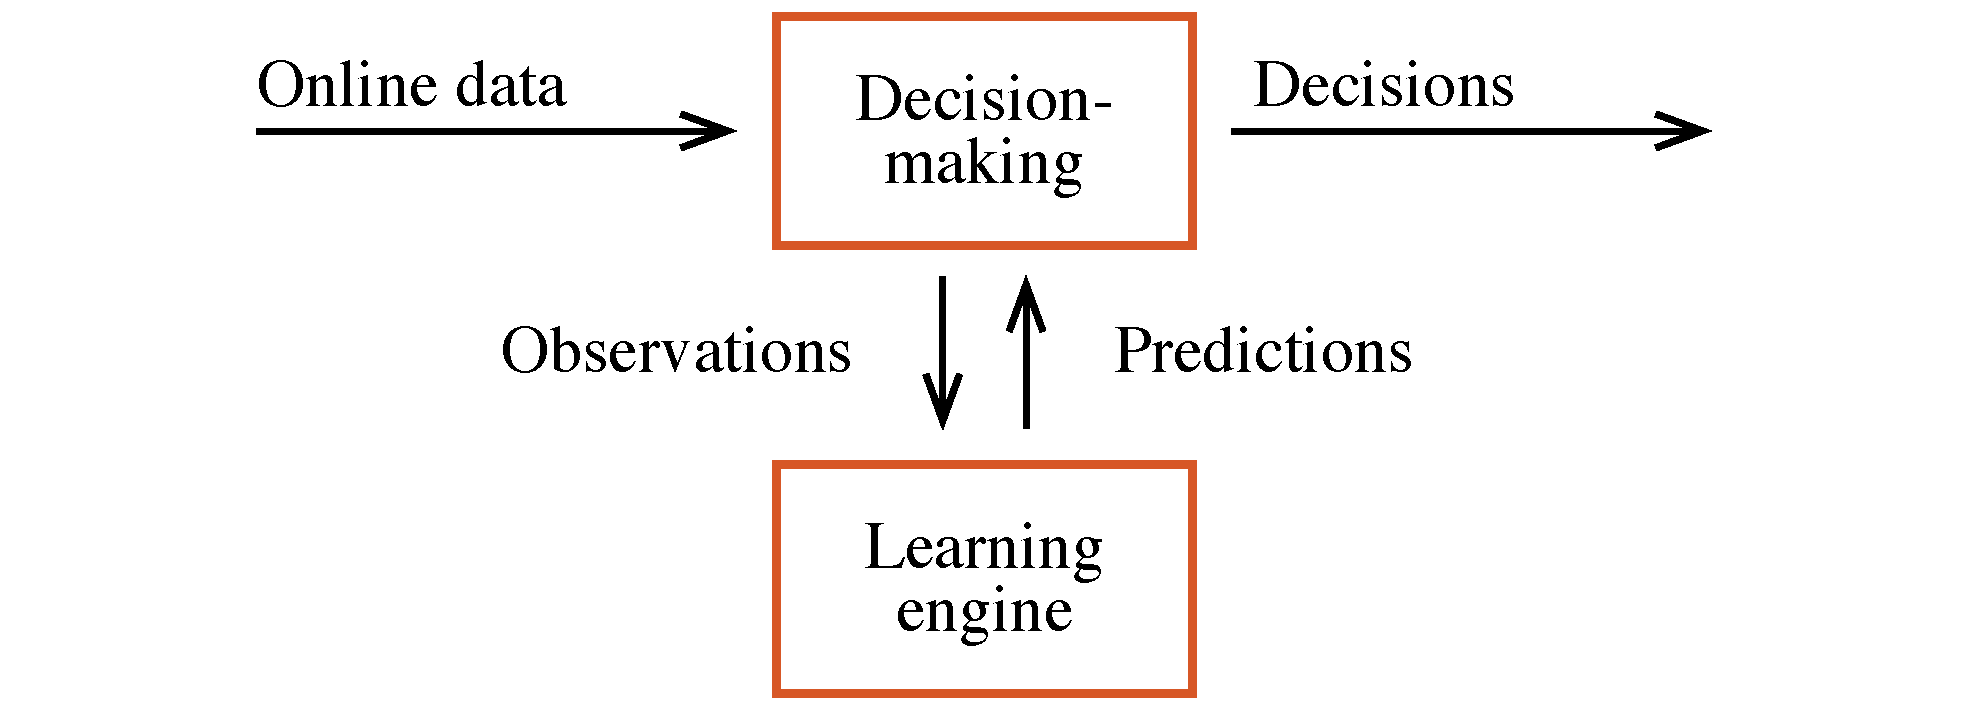
\includegraphics[width=1.0\columnwidth]{include/assets/figures/governor.pdf}
  \caption{A proactive governor of a multiprocessor system. \emph{Observations}
  refers to the data relevant for learning. \emph{Predictions} refers to the
  data that the management strategy needs to know in advance.}
  \flab{governor}
\end{figure}

Now, it should be clear that, by recording power directly, we make a trade-off:
many details related to programs' executions are discarded in order to gain
speed. What has been baked into recordings cannot be to altered at the usage
stage in general. Consider, for instance, a recording of a program that had two
cores and a shared L3 cache at its disposal. This pattern cannot be used to
replay the execution as if there was only one core. Similarly, the recording
cannot tell what would happen if the program could leverage one extra core.
